
In the era of information explosion, knowledge graph (KG) is a powerful representation for integrating billions of available relational facts, based on observational low-level knowledge in the world, to encapsulate the rich relationships of entities~\cite{ji2021survey, zhang2020aser}.
%Knowledge graphs (KG) encode structured information of entities and their rich relations, and construct billions of relational facts,
Although the massive knowledge can benefit various downstream applications, {\it e.g.} query answering~\cite{wang2021benchmarking,lin2021multi,chen2022fuzzy}, recommendation systems~\cite{wang2019kgat,wang2019multi,li2021kg4vis}, yet to better understand, exploit, and complete these underlying knowledge, it is necessary to explore the intrinsic principle of the emergence of this factual knowledge.
%it poses a great obstacle for people to generate organized cognition of the world.
For this purpose,
%To investigate the generation driving force of the massive knowledge,
the concept of meta-knowledge is proposed and defined as the \textit{knowledge about knowledge}~\cite{evans2011metaknowledge}.

% Although a typical knowledge graph may contain millions of entities and billions of relational facts, it is usually far from complete. Knowledge graph completion aims at predicting relations between en- tities under supervision of the existing knowledge graph. Knowledge graph completion can find new relational facts, which is an important supplement to relation extraction from plain texts.

% \yuanyuan{causal metaknowledge}
Current rule mining methods in the KG literature attempt to mine meta-knowledge, in the form of association rules, via correlation analysis represented by frequency analysis~\cite{galarraga2013amie,galarraga2015fast,meilicke2019anytime}.
These association rules can be used for downstream tasks such as knowledge graph completion, and question answering.
However, association does not imply causation~\cite{10.1214/ss/1177009870}.
Fortunato et al. points out that causality is necessary to identify the fundamental drivers of knowledge~\cite{fortunato2018science}.
The correlation-based method may lead to spurious correlations between the body and head of rule, which can not be generalized to new environments.

Here we take the KG-based drug repurposing task as an example (shown in Fig.~\ref{fig:rule_example}).
Given the heart disease KG as training data, traditional rule mining methods may rely on two rules \ding{172} and \ding{173} to predict the \texttt{Treat} relation.
As heart disease drugs entail similar side effects, the confidence (weight) of Rule \ding{173}, calculated based on correlation, is greater than that of Rule \ding{172} (0.7 versus 0.6).
However, the localization of the drug to the target protein produced by the disease gene, as indicated in Rule \ding{172}, is the recognized mechanism for physicians to prescribe drugs for the disease~\cite{himmelstein2017systematic}.
This phenomenon, typical of spurious correlations, is due to the scarcity of genetic information and the abundance of side-effect facts accompanying the data collection process.
Therefore, these weighted rules could produce false KG completion results as the environment shifts.
Fig.~\ref{fig:rule_example}(b) visualizes such testing process where the learned rules from heart disease KG are used to answer queries from addiction disease KG.
Both nicotine withdrawal drug (Varenicline) and psoriasis drug (Brodalumab) are known to cause the side effect suicidal tendencies.
However, the available drug for nicotine withdrawal Bupropion (which binds the gene that participates in nicotine) is not.
With the mined rules in Fig.~\ref{fig:rule_example}(a), physicians could falsely prescribe Brodalumab (Path 2) as a new treatment for nicotine withdrawal, instead of Bupropion (Path 1).
If we can learn stable relationships (such as causality) between predicted features and predicted targets, such effect of spurious correlations can be eliminated.

\begin{figure*}[t]
\centering
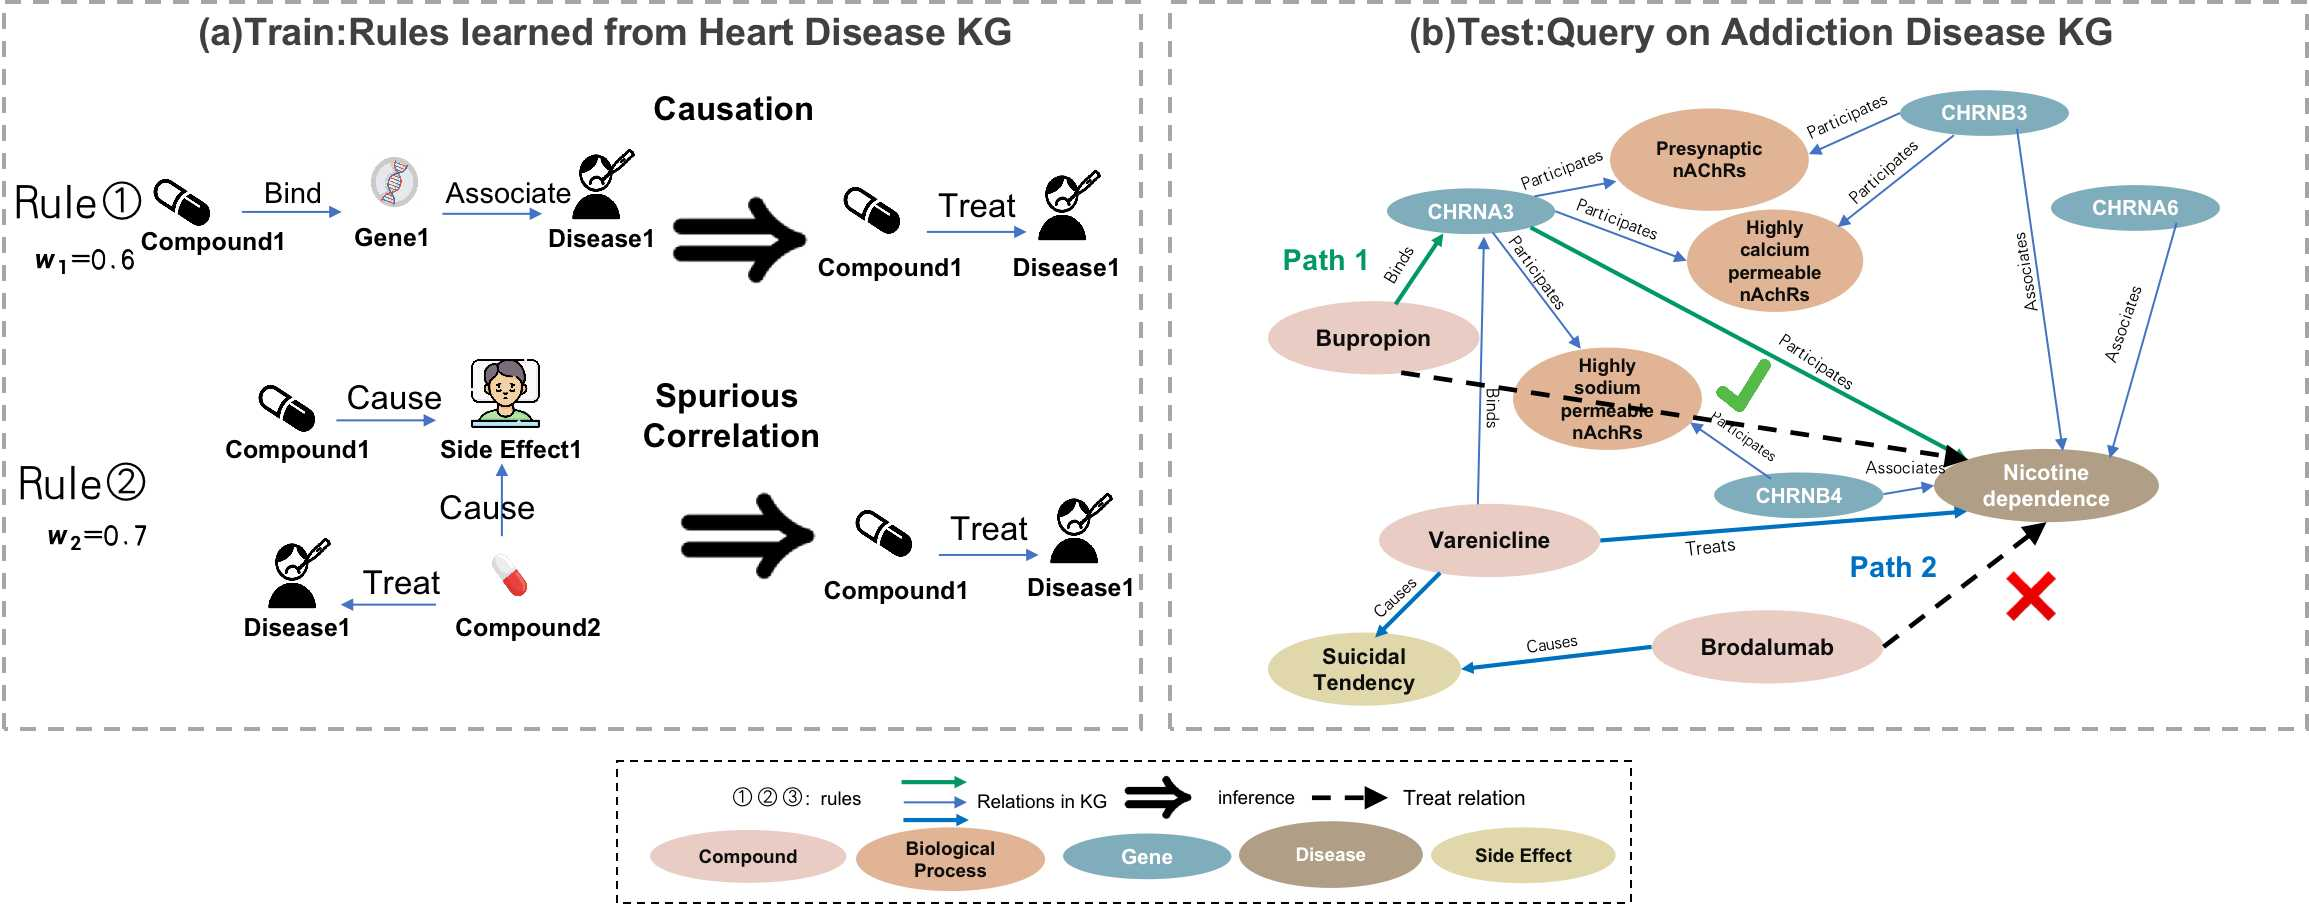
\includegraphics[width=16cm]{submissions/causal-meta-knowledge/figures/intro_case_v2.jpg}
\caption{Motivation illustration. Consider a scenario to learn rules for inferring the \texttt{Treat} relation between compounds and diseases on a heart disease KG (\emph{top}), and thereby discover novel drugs for treating nicotine addiction on an addiction disease KG (\emph{bottom}).
On the heart disease KG, drugs that treat the same disease often share the same side effects. The correlation-based approach establishes a strong spurious correlation between the shared side-effect information and the \texttt{treat} relation. In contrast, the underlying cause of the \texttt{treat} shows a weak association (Rule \ding{172}).
Therefore, when the above rule is migrated to addiction disease KG (drugs that treat the same basic kind of disease often do not have shared side effects), false prediction could be resulted (e.g., Brodalumab is more likely to be prescribed for nicotine addiction, instead of Bupropion).}
\label{fig:rule_example}
\end{figure*}

In this paper, we propose a method that learns rules from the causal perspective to ensure strong generalization ability whilst retaining decent interpretability.
Specifically, we are concerned with understanding how KG links are generated, through causal discovery.
% To improve the transferability of causal metaknowledge, we build it at the concept level termed as \textcausal rule, and it can be applied to any knowledge graphs which share the same concepts and relations.
% For example, predictive guidelines based on gene linkage information can be used not only for drug discovery in nicotine withdrawal, but also for drug discovery in COVID-19.
% In addition, the algorithm should be interpretable, which can help professionals better understand the target system.
% In addition, the algorithm should be transparent, which can help professionals better understand the target system.
There are two major challenges in this problem: 1) efficiency and 2) proper metrics.
% \textbf{Challenge 1}: \textit{How to apply causal discovery algorithms to graph data?}
% Current causal models are mainly based on quantitative tabular data, with the horizontal axis being the variables used to construct relationships and the vertical axis being the samples used for statistical analysis.
% Whereas the knowledge graph itself is a graph, which can be regarded as a sample in a way.
% Therefore how to transform the graph data into tabular representation for causal discovery is the first problem we need to deal with.\lsx{Is it necessary to say so?}
% \textbf{Challenge 1}: \textit{How to perform efficient causal rule discovery?}
For the former, the complex topological structures between massive entity pairs could induce thousand-scale rule space with barely ten relations, posing challenges for both score-based and constraint-based causal discovery approaches.
The complexity of the constraint-based technique increases exponentially with the number of nodes, whereas the score-based approach creates an NP-hard problem~\cite{le2016fast}.
% \textbf{Challenge 2}:  \textit{How to use causal information for link prediction?}
For the latter, rule-mining algorithms generally require specific metrics, such as support rate, as the weights for inference.
Therefore, we also need to design a metric to measure the strength of each causal relationship.

In this work, we first formulate causal meta-knowledge with the concept of \textit{causal rule}, on which we further introduce several constraints to reduce the search space.
Then, we propose the CMLP (Causal Metaknowledge-based Link Prediction) algorithm, which integrates efficient causal rule discovery approach and causation-based link prediction method.
Specifically, we first introduce the concept of rule-induced variable, which uses relation paths to describe the topological structure of entities, and map the graphs into quantified samples with the designed assignment function.
Further, we observe that the whole causal structure is not necessary for specific link prediction task, but only the part of the structure related to the predicted relation.
Therefore, we design an efficient method based on $d$-seperation to achieve local causal discovery.
Meanwhile, the causal strength based on conditional dependence can also be generated as the weights of learned causal rules.
Finally, the predictions can be ranked from weighted causal rules.
% Also note that there are some similarities between existing rule-based methods and the proposed CMLP, we eliminate the spurious correlations brought by common cause in the causal discovery process, thus guaranteeing the consistency between inference weights and causal strengths.\lsx{Left out}

% In summary, the main contributions of this work are as follow:
% \begin{itemize}
% \item This work introduces CMLP that learns a link predictior based on discovering causal metaknowledge.
% \item This work introduces CMLP that learns a link predictior based on discovering causal metaknowledge
% \item CMLP outperforms competitive baselines on link prediction tasks under Out-of-Distribution (OoD) setting. Furthermore, we analyze the learned metaknowledge to get some insights on the physical mechanism of the applications.

% \end{itemize}

\noindent
\textbf{Contributions.} Our main contributions can be summarized as follows: {(\it i)} This is the first work that aims at improving link prediction in KG by causal inference to eliminate the effect of spurious correlation, as evidenced in traditional methods. {(\it ii)} This work introduces CMLP that learns a link predictor based on discovering causal meta-knowledge. {(\it iii)}  CMLP outperforms other competitive baselines on link prediction tasks under Out-of-Distribution (OoD) setting. Furthermore, we analyze the learned meta-knowledge for insights on the mechanism of the applications. 